\chapter{Population Synthesis}\label{ch:synthesis}

    In order to derive meaningful conclusions about the outflows from NS mergers, given
    the models described in Chapter \ref{ch:introduction}, it was necessary to carry out
    population synthesis studies. In these studies, population models which are
    physically or observationally motivated are taken from the literature and used to
    compute the statistical properties of outflows from NS binaries synthesized from
    these models. If no confident or relevant model was yet described in literature,
    physically motivated ans\"{a}tze are used (see for example,
    \S\S\ref{sub:spin-dists}).\\
    In each study which uses (slightly) different population models, 10$^5$ samples were
    drawn from the relevant parameter distributions. Using these as inputs, the expected
    outflows were calculated using the fit formulae described in Chapter
    \ref{ch:introduction} for the outflows from NSBH mergers.\\
    In this chapter, the various population models are briefly described along with
    their pertinence. Furthermore, preliminary checks for the population synthesis code
    are also discussed, which help verify the consistency of the code with theoretical
    results.

\section{Black Hole Population Models}\label{sec:bh_pop}

    \subsection{Mass, $M_{BH}$}
        The masses of the black holes was sampled from the \textsc{truncated} mass
        distribution from \cite{abbott_2020B}. The distribution `produces' black holes
        with masses between 3--100 M$_\odot$ (as can be seen from Fig.
        \ref{fig:bh_mass_gwtc2}).  However, NS binaries with extremely massive ($M_{BH}
        > 20 M_\odot$) black holes will not produce any appreciable EM emission, due to
        the NS companion plunging into the black hole directly. For this reason, an
        upper limit of 20 M$_\odot$ is imposed on the black hole masses sampled in the
        population synthesis code.

        \begin{figure}[H]
            \centering
            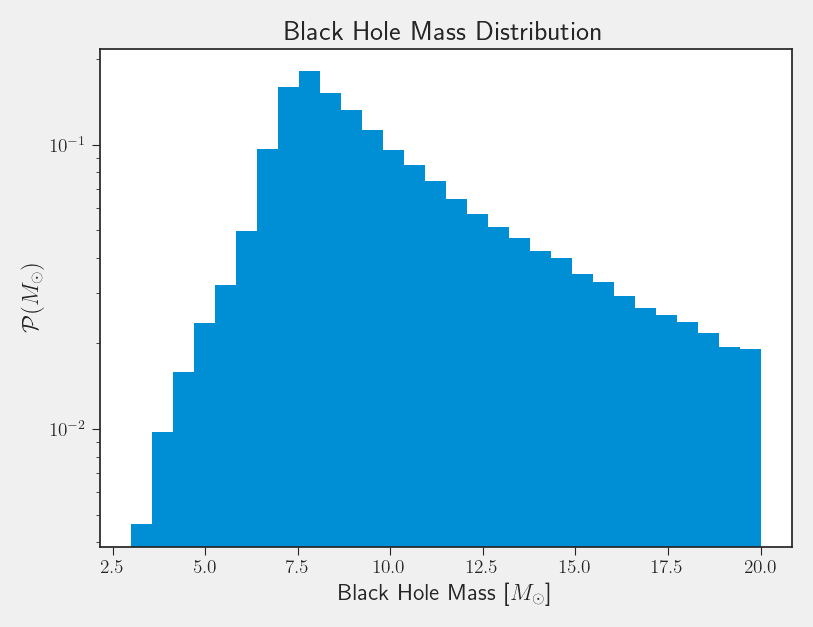
\includegraphics[width=0.8\linewidth]{bh_mass}
            \caption[Black hole mass distribution with upper limit]
            {
                Black hole mass distribution as used in the current report, with an
                upper limit of 20 M$_\odot$.
            }
            \label{fig:bh_mass}
        \end{figure}

        \begin{figure}
            \centering
            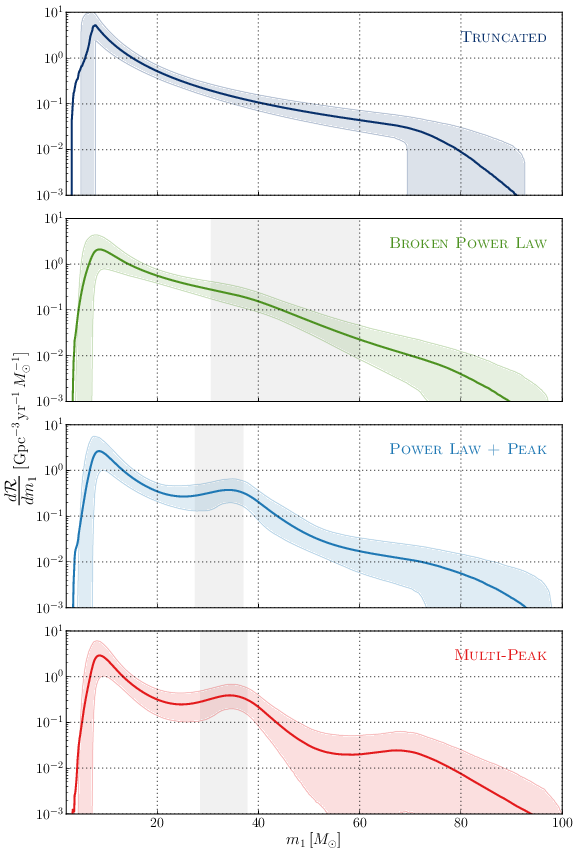
\includegraphics[width=0.9\linewidth]{bh_mass_gwtc2}
            \caption[Black hole mass distributions from GWTC-2]
            {
                Black Hole Mass Distributions from \cite{abbott_2020B}. In the current
                study, the \textsc{truncated} mass distribution with an upper limit at
                20 M$_\odot$, since more massive black holes would not produce
                significant EM emission when in a merging NSBH binary.
            }
            \label{fig:bh_mass_gwtc2}
        \end{figure}

    \subsection{Spin, $\chi_{BH}$}\label{sub:spin-dists}
        The spins of the black holes are sampled from the \textsc{default} distribution
        given in \cite{abbott_2020B}. This distribution is essentially a Beta
        distribution, which ensures that the spin parameters sampled from this
        distribution remain within [0, 1).\\
        However, since there have been not many confident NSBH merger detections in the
        GW regime, this distribution is largely derived from observing BBH mergers, and
        thus may not represent the true spin distribution of black holes in NSBH
        binaries.  To circumvent this, the following ans\"{a}tze are used to probe the
        effect of the spin distribution on the EM outflows:

        \begin{figure}[H]
            \centering
            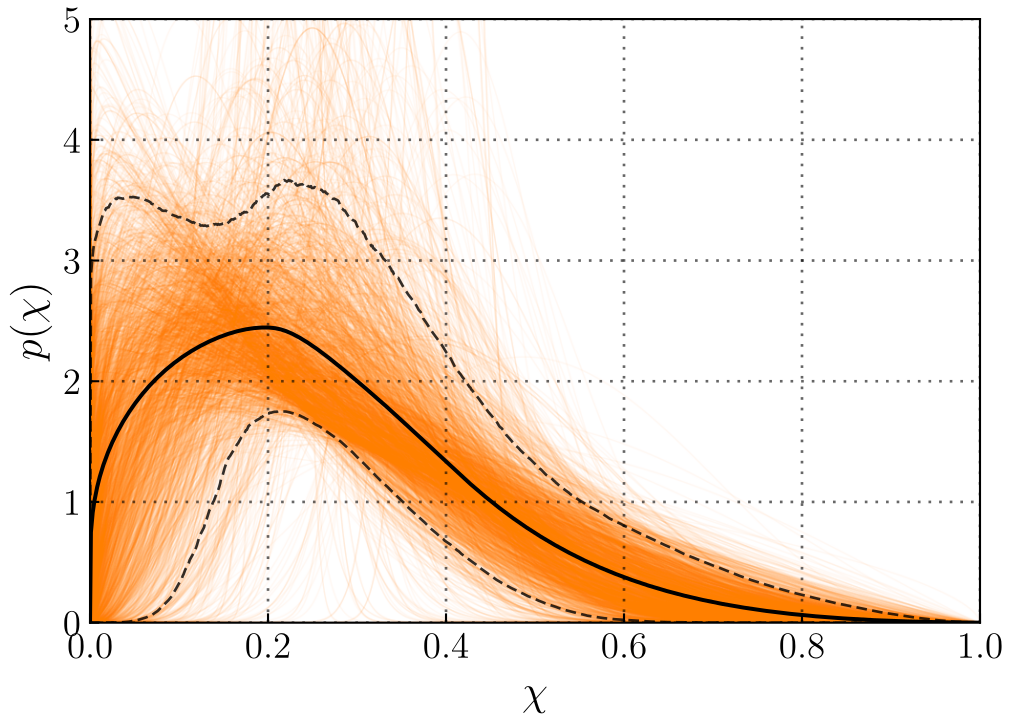
\includegraphics[width=0.8\linewidth]{bh_spin_gwtc2}
            \caption[Black hole spin distribution from GWTC-2]{
                Beta distribution for the  black hole spin from \cite{abbott_2020B}.
                Here the light traces are samples from the posterior distribution,
                whereas the solid black line is the posterior probability distribution
                for $\chi_{BH}$. Dashed black lines mark the 90\% quantiles for the
                same.
            }
            \label{fig:bh_spin_gwtc2}
        \end{figure}


        \begin{itemize}

            \item Uniform spin distribution: here $\chi_{BH} \sim \mathcal{U}(0, 1)$.
                Note also that this distribution will have a \emph{higher number of high
                spin samples} as compared to the \textsc{default} distribution
                considered above.

                \begin{figure}[H]
                    \centering
                    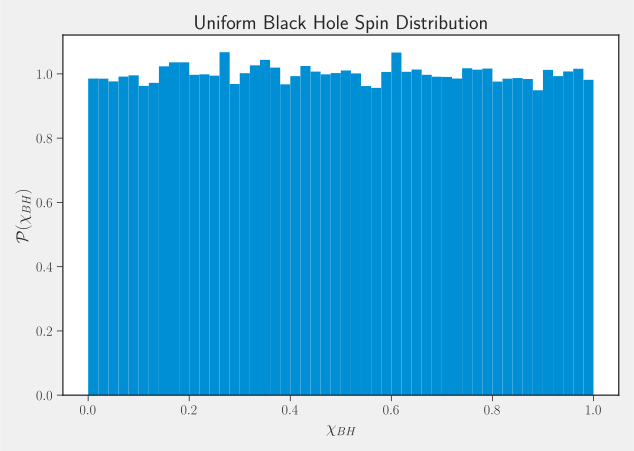
\includegraphics[width=0.7\linewidth]{unif_dist}
                    \caption[Uniform Black Hole Spin Distribution]{
                        A realisation of the uniform black hole spin distribution
                        considered here.
                    }
                    \label{fig:unif_dist}
                \end{figure}

            \item Gaussian spin distributions: here $\chi_{BH} \sim \mathcal{N}(\mu,
                \sigma)$, but samples outside of [0, 1) are not considered. Here, $\mu,
                \sigma$ represent the mean and standard deviation, respectively, of the
                Gaussian distribution. For simplicity and to cover a representative
                number out of all the possible distributions, samples were taken from
                $\mathcal{N}(0.2, 0.2)$, $\mathcal{N}(0.5, 0.2)$ and $\mathcal{N}(0.7,
                0.2)$. These represent distributions concentrated around low, medium and
                high spins respectively.

                \begin{figure}[H]
                    \centering
                    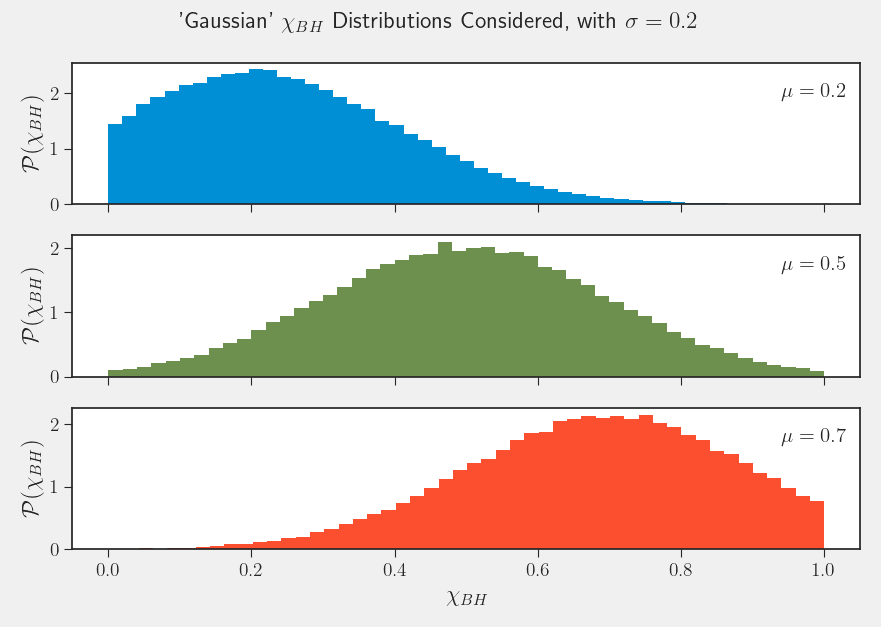
\includegraphics[width=0.8\linewidth]{gauss_dists}
                    \caption[Gaussian Black Hole Spin Distributions]{
                        Realisations of the various `Gaussian' black hole spin
                        distributions considered here.
                    }
                    \label{fig:gauss_dists}
                \end{figure}

        \end{itemize}


\section{Neutron Star Population Models}\label{sec:ns_pop}

    In order to reduce the number of variables in the problem, the masses and radii of
    all neutron stars in the population was set to 1.4 M$_\odot$ and 11 km respectively.
    These values correspond to the median values inferred for GW170817 (see
    \cite{abbott_2018}). Also, the spins of all neutron stars synthesized was set to 0,
    since it is assumed that sufficient amount of time would have passed between the
    formation of the binary and merger, allowing for the neutron star to spin down such
    that $\chi_{NS} \sim 0$.\\
    Additionally, the tidal deformability of the neutron stars, $\Lambda_{NS}$ was set
    using the C-love relation (see \cite{yagi_2017}). In order to do this, the
    compactness of the neutron stars, $C_{NS}$ was computed using the relation :

    \begin{equation}
        C_{NS} = \dfrac{G M_{NS}}{R_{NS} c^2}
    \end{equation}

    Where $M_{NS}$, $R_{NS}$ are the mass and radius of the neutron star, G is the
    universal gravitational constant and c is the speed of light.  Finally, the tidal
    deformability is computed by solving the C-Love relation :

    \begin{equation}
        C_{NS} = \sum_{k=0}^{2} a_k (\ln \Lambda_{NS})^k
    \end{equation}

    Where $\Lambda_{NS}$ is the tidal deformability of the neutron star, and $a_k$ are
    the fit coefficients as given in \cite{yagi_2017}.

\section{Spatial Distribution and Orientation of Samples}\label{sec:space_dist}

    \subsection{Constant comoving volume distribution}

        The simulated events whose component mass and spin distributions were described
        in \S\ref{sec:bh_pop}--\ref{sec:ns_pop} are distributed in 3D space such that
        their number density is constant in comoving volume.\\ For this, firstly the
        latitudinal ($\theta$) and longitudinal ($\phi$) angles are sampled such that
        $\cos \theta \sim \mathcal{U}(-1, 1)$ and $\phi \in \mathcal{U}(0, 2\pi)$, i.e.
        such that they are uniform on a unit sphere. As for the comoving distance
        distribution $\mathcal{P}(D_c)$, consider the probability of an event lying in
        an infinitesimal shell of width d$D_c$ at a comoving distance $D_c$.  Then it
        can be seen that:

        \begin{equation}
            \mathcal{P}(D_c) dD_c \propto D_c^2 dD_c \Rightarrow
                \boxed{\mathcal{P}(D_c) = \alpha D_c^2}
        \end{equation}

        Where $\alpha$ is the constant of proportionality. In the local universe, it can
        be safely assumed that $D_c \approx D_L$, where the latter is the luminosity
        distance.  However from the fact that the GW network SNR $\rho \propto
        D_L^{-1}$, it can also be seen that:

        \begin{align}
            \mathcal{P}(\rho) &= \mathcal{P}(D_L)
                                  \Big \lvert \dfrac{dD_L}{d\rho} \Big \rvert
                                  \nonumber\\
                              &= \mathcal{P}({D_c})
                                  \Big \lvert \dfrac{dD_c}{d\rho} \Big \rvert
                                  \nonumber\\
                              &\propto \dfrac{1}{\rho^2} \dfrac{1}{\rho^2}
                                  = \dfrac{1}{\rho^4} \nonumber\\
            \Rightarrow \mathcal{P} (\rho) &= \dfrac{\beta}{\rho^4}
        \end{align}

        Once the SNR detection threshold\footnote{
            This is defined such that any event with a GW network SNR greater than the
            detection threshold will be considered a detection.
        } ($\rho_{th}$) is set, the normalization constants can be computed as follows:

        \begin{align}
            \int_0^{D_{c, max}}
                \mathcal{P}(D_c) dD_c &= \int_0^{D_{L, max}} \mathcal{P}(D_L) dD_L \\
                                      &= \int_\infty^{\rho_{th}} \mathcal{P}(\rho)
                                          d\rho \\
                                      &= 1
        \end{align}

        This gives:

        \begin{align}
            \label{eq:lum_dist}
            \mathcal{P}(D_L) = 3 \dfrac{D_L^2}{D_{L, max}}
                                 \Leftrightarrow
            \mathcal{P}(\rho) = 3 \dfrac{\rho_{th}^3}{\rho^4}
        \end{align}

        Where $D_{L, max}$ is the luminosity distance corresponding to the detection
        threshold. As an example, for the Advanced LIGO/VIRGO design configuration and a
        network SNR threshold of 10, $D_{L, max} \approx 1123$ Mpc.\\
        Using Eq. \ref{eq:lum_dist}, samples are drawn from the luminosity distance
        distribution and using the previous samples for $\theta$ and $\phi$, events are
        distributed in 3D space such that the number density of events is constant in
        the comoving volume.

    \subsection{Orientation of Events}\label{sub:orientation_of_events}

        The orientation of NSBH binaries with respect to the line-of-sight is prescribed
        using the inclination angle, $\iota$ and the polarization angle of the incoming
        GW signal, $\psi$. These are distributed in the population synthesis such that
        $\cos\iota \sim \mathcal{U}(-1, 1)$ and $\psi \sim \mathcal{U}(0, 2\pi)$, from
        which samples are drawn for individual events.

\section{Validation of Population Synthesis Code}\label{sec:popsyn_validation}

    With the population models for the binary component parameters as described in the
    previous sections, 10$^5$ samples are drawn from each model to generate a
    population.  These populations will majorly differ in the black hole spin
    distribution and are thus distinguished by that very factor.\\
    Given these populations, several checks were carried out to confirm the consistency
    of the underlying models and the population generated, with the use of (both EM and
    GW) theoretical results. The rationale behind these checks and the results are given
    in the following sections.

    \subsection{GW Checks}\label{sub:gw_checks}

        Firstly, for the samples generated, the optimal GW SNR corresponding to the
        binary parameter combinations was computed. This was done by using the
        restricted post-Newtonian (PN) waveform (RWF; see \cite{cutler_1994}) as the GW
        template for the expected strain signal corresponding to an actual merger event.
        For this case, the template is given using the frequency domain representation:

        \begin{equation}
            \tilde{h}(f) = \mathcal{A}f^{-7/6}e^{i\phi(f)}
            \label{eq:rwf}
        \end{equation}

        Where $\mathcal{A} = \sqrt{5/96}\pi^{-2/3} \mathcal{M}$ is the amplitude,
        $\mathcal{M} = M \eta^{5/3}$ is the chirp mass, $M$ is the total mass, $\eta =
        \frac{m_1 m_2}{M}$ is the symmetric mass ratio, and $\phi(f)$ is the frequency
        domain GW phase function. With the RWF template, the PN approximations made
        ensure maximum accuracy with respect to the phase but ignore the PN corrections
        to the amplitude of the gravitational waveform. However, this trade-off is
        beneficial since accurately tracking the phase evolution is vital for
        inferring the binary masses (\cite{poisson_1995}), which helps in classifying
        which type of compact binary coalescence (CBC) the incoming signal corresponds
        to. For such a template, the optimal SNR at a detector with a noise power
        spectral density (PSD) $S_h(f)$, is computed as:

        \begin{equation}
            \rho = \sqrt{
                            4\int_0^\infty
                            \dfrac{\lvert \tilde{h}(f) \rvert^2}{S_h(f)}
                            df
                        }
            \label{eq:rho}
        \end{equation}

        Substituting the form of $\tilde{h}(f)$ from Eq. \ref{eq:rwf}, one obtains:

        \begin{multline}
            \label{eq:rwf_optsnr}
            \rho(m_1, m_2, D_L, \theta, \phi, \psi, \iota) =
                \Big\{
                    4 \dfrac{\mathcal{A}^2}{D_L^2}
                    \Big[
                        F_{+}^2(\theta, \phi, \psi)(1 + \cos^2 \iota)^2 + \\
                        4 F_{\times}^2(\theta, \phi, \psi) \cos^2 \iota
                    \Big]
                     I(M)
                 \Big\}^{1/2}
        \end{multline}

        Where $F_{+, \times}(\theta, \phi, \psi)$ are the antenna pattern functions for
        the `plus' and `cross' GW polarizations, and the four angles $\{\theta, \phi,
        \psi, \iota\}$ prescribe the location and orientation of the source with respect
        to the detector. Also, $I(M)$ is the frequency integral given by:

        \begin{align}
            I(M) &= \int_0^\infty \dfrac{f^{-7/3}}{S_h(f)} df \\
                 &\approx \int_{f_{low}}^{f_{LSO}} \dfrac{f^{-7/3}}{S_h(f)} df
            \label{eq:freq_integral}
        \end{align}

        Where $f_{low}$ corresponds to the seismic cut-off in the detector noise PSD
        curve, and $f_{LSO}$ corresponds to the frequency at the last stable orbit for a
        black hole of total mass M, which under the PN approximation is $f_{LSO} =
        (6^{3/2} \pi M)^{-1}$.\\
        For each sample in the various populations, the optimal SNR was computed using
        the above formulae with the aid of the PyCBC (\cite{pycbc}) Python package along
        with the LALSimulation C libraries (\cite{lalsuite}). Using the computed SNRs,
        it was verified that the events \textit{are} distributed in luminosity distance
        (and thus SNR) as expected from \ref{eq:lum_dist}. This is given in
        Fig. \ref{fig:rho_dist}. Note that in order to verify this relation, one must
        only consider the events whose network SNR is above the threshold SNR chosen (in
        this case, 10).\\

        \begin{figure}[H]
            \centering
            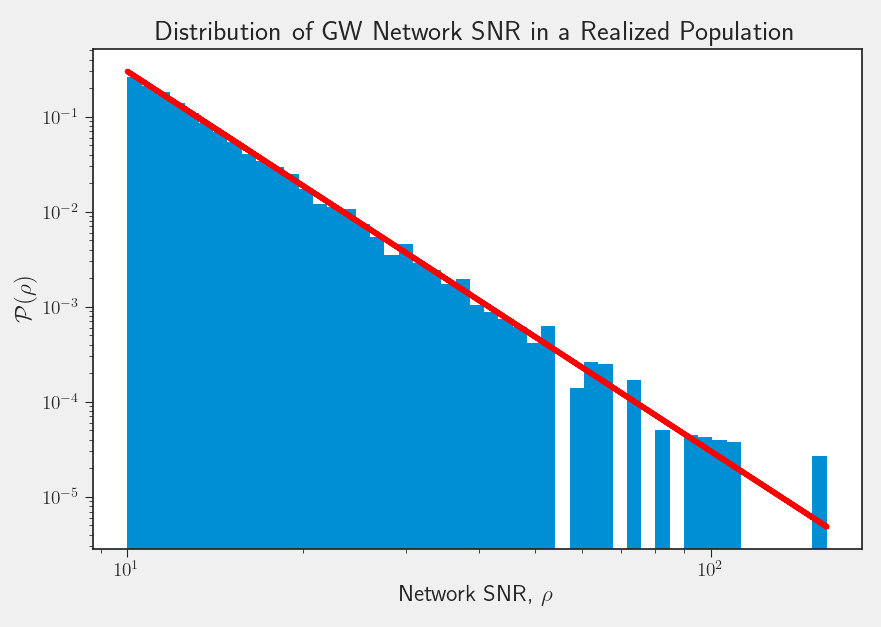
\includegraphics[width=0.8\linewidth]{rho_dist}
            \caption[Distribution of GW network SNR]
            {
                Distribution of GW network SNR, from a particular realisation of a
                population with standard assumptions about binary parameters, and a
                uniform spin distribution. The red line is the curve given by
                theoretical considerations, which for a threshold SNR of 10, corresponds
                to $f(\rho) = 3\rho_{th}^3 / \rho^4 = 3000 / \rho^4$.
            }
            \label{fig:rho_dist}
        \end{figure}


        Furthermore, from Eq. \ref{eq:rwf_optsnr}, the GW network SNR is higher in value
        if:

        \begin{itemize}

            \item The merger `event' is closer by, i.e. $D_L$ is low.

            \item The binary merges with the orbital plane face on, i.e. $\iota$ is low

            \item \emph{Both} $D_L$ and $\iota$ are low, although this is a small part
                of the $D_L-\iota$ parameter space and hence is less probable.

        \end{itemize}

        This implies a connection between the two parameters, and indeed this $D_L-\iota
        $ connection is well studied in the literature (see \cite{schutz_2011} \&
        \cite{seto_2015} for discussions on the same). This relation is also important
        for joint EM-GW observations since the EM signals are inversely proportional to
        the distance to a binary merger which may produce the prompt emission, whereas
        the GW signal is sensitive to the inclination angle. This behaviour of the GW
        SNR was verified to hold within the population generated, which is shown in Fig.
        \ref{fig:dl_iota_correlation}. Note that some parts of the $D_L - \iota$
        parameter space are not at all populated by the samples, which reaffirms the
        fact that distant, edge-on mergers are disfavoured when such systems are being
        explored via GW.

        \begin{figure}[htpb]
            \centering
            \includegraphics[width=0.8\linewidth]{iota_dl_colorcoded}
            \caption[$D_L-\iota$ correlation in the population]{
                Plot of the luminosity distance v/s the inclination angle for events in
                the population, colour coded by the SNR. Note that only events whose SNR
                > 10 (the SNR threshold) are considered here.  This shows that the
                generated population also exhibits the relation as expected from theory.
            }
            \label{fig:dl_iota_correlation}
        \end{figure}

    \subsection{EM Checks}\label{sub:em_checks}

    The only EM component which has to be validated is the code which imposes the jet
    structure (Eq. \ref{eq:dE_dOmega} -- \ref{eq:eiso}), once the energetics of the jet
    are computed via Eq. \ref{eq:e_kin_jet} -- \ref{eq:Omega_h}.\\
    In order do this, one extracts the $\theta_v$ samples from the generated population,
    which can be done using the relation $\theta_v = \min(\iota, \pi - \iota)$. Then, a
    common baseline is achieved by setting the value of $E_{kin, jet} = 10^{49} \text{
    erg}$ for all samples, regardless of the actual value if the binary parameters were
    to be taken into consideration. This is necessary to \emph{remove} the variation of
    the structure with the intrinsic jet energetics, which is intimately related to the
    binary parameters.\\
    Then with this constraint applied, the value of $E_{iso}(\theta_v)$ is computed
    using Eq.  \ref{eq:dE_dOmega} -- \ref{eq:eiso}. It is seen from Fig.
    \ref{fig:jet_struct} that jet structure is being imposed correctly and according to
    what is expected from theory.

    \begin{figure}[H]
        \centering
        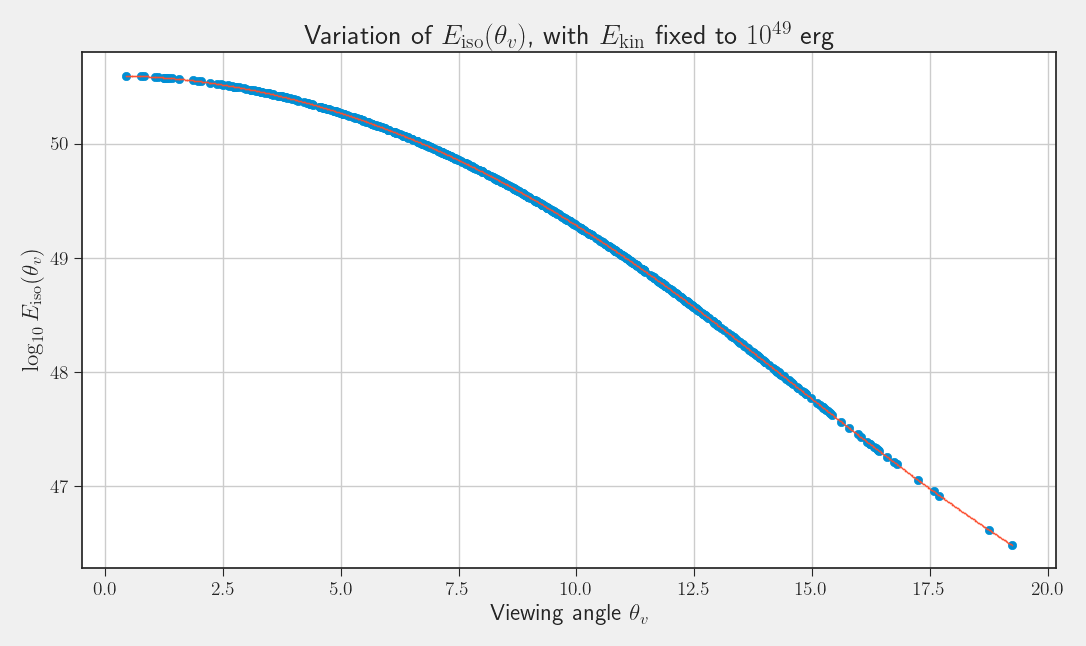
\includegraphics[width=0.8\linewidth]{jet_struct}
        \caption[Validation of the jet structure code]
        {
            Validation of the jet structure code, using the process mentioned in text.
            The blue scatter points are the values computed for $E_{iso}(\theta_v)$ for
            parameters from a population with $E_{kin, jet}$ set to $10^{49}$ erg,
            whereas the red line is that computed from theory for a jet with the same
            kinetic energy.
        }
        \label{fig:jet_struct}
    \end{figure}

    One additional check was performed to confirm the distribution of simulated, jet
    launching binary mergers. The number of mergers which launched a jet with a fluence
    greater than some particular value ($\mathcal{N}(>\mathcal{F})$) was plotted, as a
    function of the particular fluence value($\mathcal{F}$).\\
    If the jet structure and spatial distribution codes were working to mimic what is
    observed in reality, the resulting structure should be isotropic but inhomogeneous,
    since the sources would be cosmological in nature but appear isotropically
    distributed in the local universe. As for the expected behaviour of $\mathcal{N}(>
    \mathcal{F})$, it would behave as $\mathcal{F}^{-1.5}$ for large values of
    $\mathcal{F}$, but would significantly deviate from this behaviour
    for smaller values of $\mathcal{F}$.

    \begin{figure}[H]
        \centering
        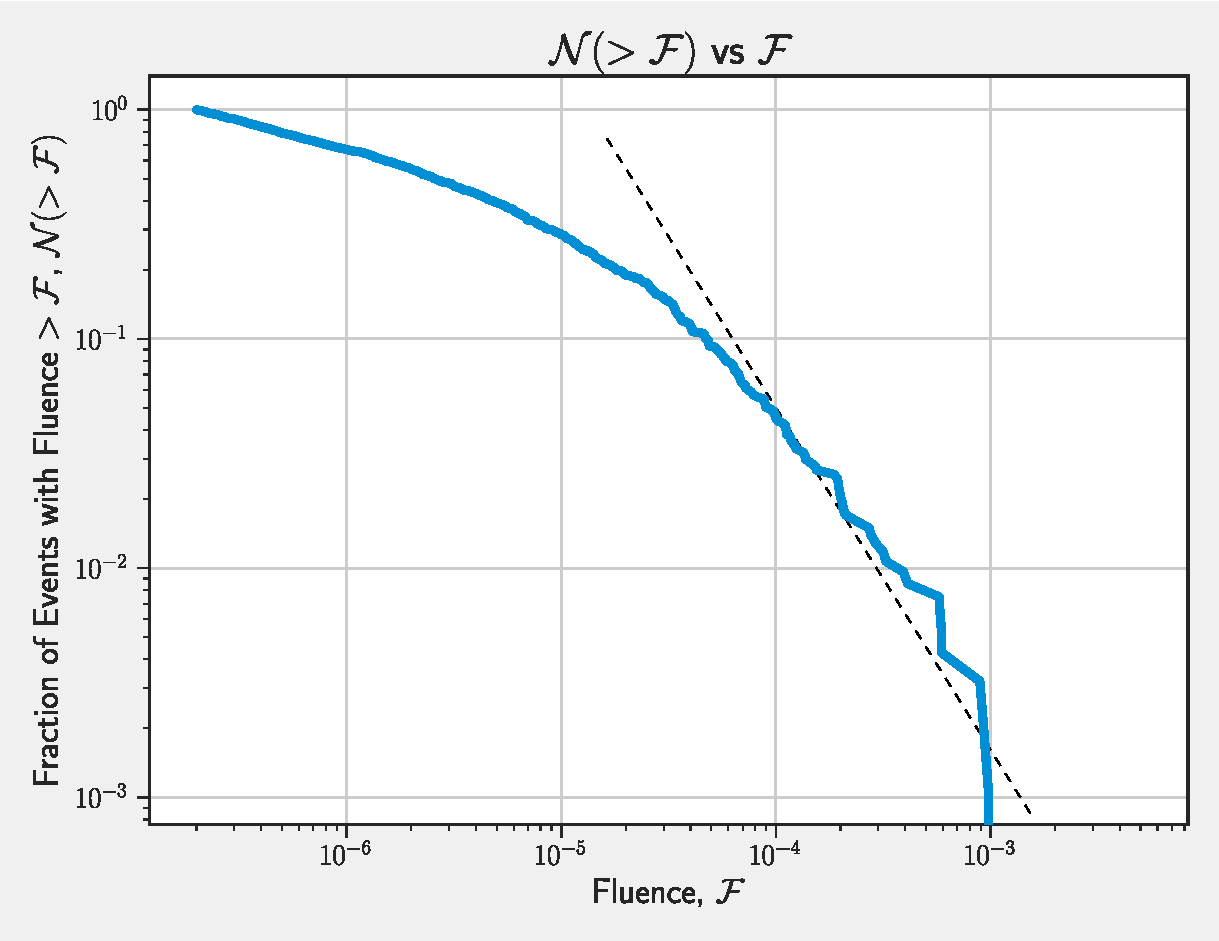
\includegraphics[width=0.9\linewidth]{number_fluence}
        \caption[Variation of $\mathcal{N}(> \mathcal{F})$ with $\mathcal{F}$]{
            Variation of $\mathcal{N}(> \mathcal{F})$ with the fluence $\mathcal{F}$.
            Note the significant deviation of this function from the $\sim
            \mathcal{F}^{-1.5}$ behaviour at lower values of the fluence.
        }
        \label{fig:number_fluence}
    \end{figure}

    From Fig. \ref{fig:number_fluence}, it is seen that the distribution of simulated
    mergers which launch a jet mimics the observed distribution of SGRBs in the
    Universe, and so the jet structure and spatial distribution codes are satisfactory.

    As an additional check for the jet structure and energetics code, a few prototypical
    binary mergers are considered, where each prototype is identified by the mass ratio,
    $\mathcal{Q}$, which is varied as $\mathcal{Q} = \frac{3}{1.4}, \frac{5}{1.4},
    \frac{10}{1.4}$. The variation of the fluence with the black hole spin, $\chi_{BH}$
    and the viewing angle, $\theta_v$ is what is studied in each prototypical case.
    These are given in Figs. \ref{fig:fluence_thetav+spin(3)} --
    \ref{fig:fluence_thetav+spin(5)}.

    \begin{figure}[H]
        \centering
        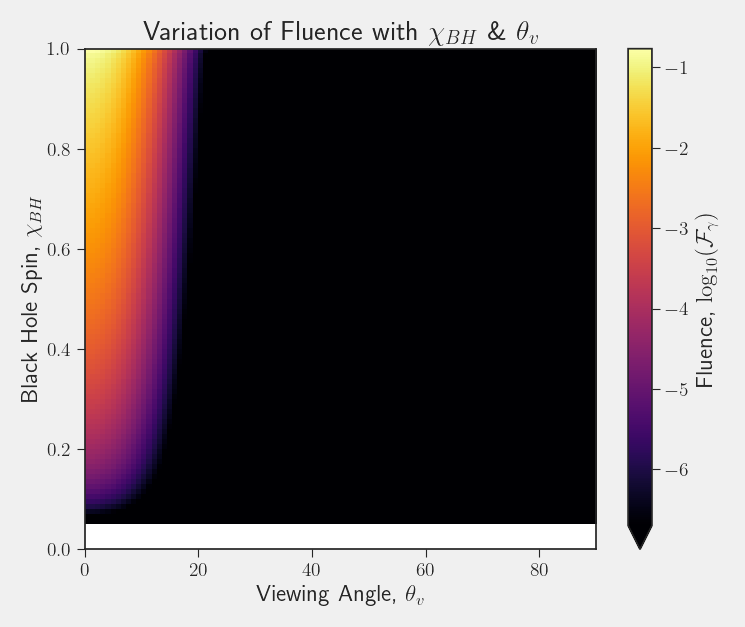
\includegraphics[width=0.8\linewidth]{fluence_thetav+spin(3)}
        \caption
        [
            Variation of $\mathcal{F}(\chi_{BH}, \theta_{v})$ for a $\mathcal{Q}=3:1.4$
            NSBH binary merger
        ]
        {
            The variation of fluence with the viewing angle and the black hole spin for
            a binary merger with a mass ratio of $\mathcal{Q}=3:1.4$. Here the regions
            of the $\chi_{BH}-\theta_v$ parameter space in white are those regions where
            no disc is produced, and hence the outgoing fluence is 0.
        }
        \label{fig:fluence_thetav+spin(3)}
    \end{figure}

    A few important points are readily visible from careful observation of the Figs.
    \ref{fig:fluence_thetav+spin(3)} -- \ref{fig:fluence_thetav+spin(5)}, which will be
    useful for the discussion in subsequent chapters:

    \begin{itemize}

        \item The higher the mass ratio of the merging NSBH system, the lower the
            probability for a jet to be launched. This is because the inspiralling NS
            plunges into the BH more often than not, thus undergoing little to no tidal
            disruption. Thus, the possibility of disc formation, and thus jet launching
            is very low in very asymmetric binaries.

        \item With asymmetric binary mergers, only if the black hole spin is high enough
            will there be any possibility of jet launching. This is because with a high
            enough black hole spin, the inspiralling NS can become tidally disrupted,
            and thus a massive disc can be formed using which a jet can be launched.
            However, it is highly unlikely that such high black hole spins are actually
            physical.

    \end{itemize}

    \begin{figure}[H]
        \centering
        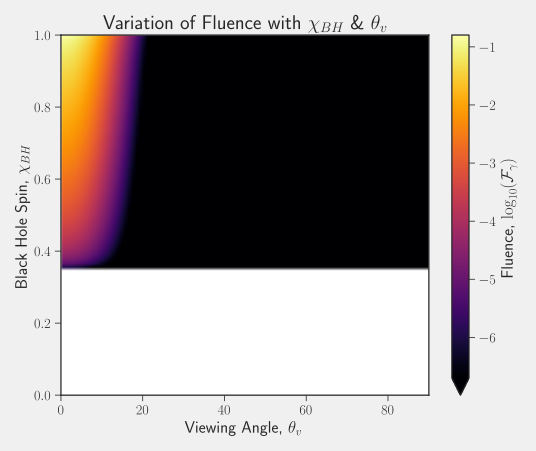
\includegraphics[width=0.8\linewidth]{fluence_thetav+spin(5)}
        \caption
        [
            Variation of $\mathcal{F}(\chi_{BH}, \theta_{v})$ for a $\mathcal{Q}=5:1.4$
            NSBH binary merger
        ]
        {
            The variation of fluence with the viewing angle and the black hole spin for
            a binary merger with a mass ratio of $\mathcal{Q}=5:1.4$. Note that in this
            case the region where a disc is not produced is a much larger fraction of
            the parameter space, compared to Fig.\ref{fig:fluence_thetav+spin(3)}.
        }
        \label{fig:fluence_thetav+spin(5)}
    \end{figure}

    Thus, from Figs.\ref{fig:fluence_thetav+spin(3)} --
    \ref{fig:fluence_thetav+spin(5)}, it can be seen that symmetric binary mergers will
    produce much brighter jets for a given black hole spin, and these jets will be seen
    out to higher viewing angles. This fact will be useful while discussing the analysis
    of the various populations synthesized, along with their EM/GW/joint
    detectability.  Furthermore, from these figures, it is also verified that the code
    which imposes the jet structure and energetics is working correctly, since these
    conclusions about the EM detectability of NSBH binary mergers are the ones
    corroborated by literature as well (see \ref{sec:nsbh} for a brief overview of the
    literature discussing these results).

    \begin{figure}[ht]
        \centering
        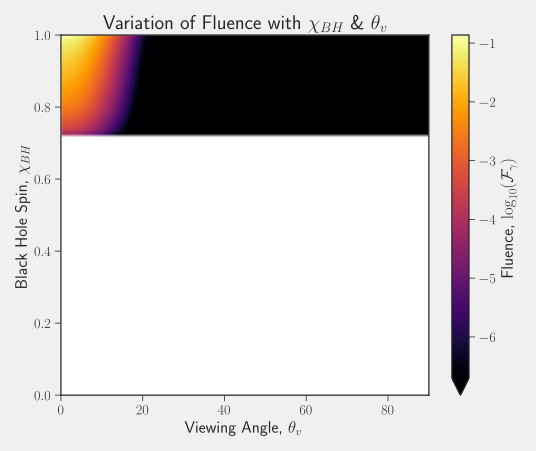
\includegraphics[width=0.8\linewidth]{fluence_thetav+spin(10)}
        \caption
        [
            Variation of $\mathcal{F}(\chi_{BH}, \theta_{v})$ for a $\mathcal{Q}=10:1.4$
            NSBH binary merger
        ]
        {
            The variation of fluence with the viewing angle and the black hole spin for
            a binary merger with a mass ratio of $\mathcal{Q}=10:1.4$. Here the region
            of parameter space where the jet is launched is extremely restricted, as the
            NSBH binary in question is extremely asymmetric in its masses.
        }
        \label{fig:fluence_thetav+spin(10)}
    \end{figure}

\section{Summary}

    In this chapter, the various populations that will be used to probe the EM
    counterparts of NSBH mergers were introduced. Along with this, a summary of the
    various tests carried out was given, wherein the tests made sure that the internal
    codes that compute GW SNRs, calculate jet energetics (from formulae derived as fits
    to numerical relativity simulations), impose jet structures etc., gave preliminary
    results which align with the theoretical results.\\
    In the coming chapters, the framework set up in this and the previous chapters for
    the synthesis of the populations, will be used to analyse the generated populations
    and the resulting NSBH merger events will be used to derive results about the
    properties of these binary mergers, and their subsequent prompt EM counterparts.
